\setcounter{rownumber}{0}
\singlespacing
\chapter{Brillouin-Induced Raman Modes and Device Exploration}
\label{ch:Raman}
\acresetall

\doublespacing

%%%%%%%%%%%%%%%%%%%%%%%%%%%%%%%%%%%%%%%%%%%%%%%%%%%%%%%%%%%%%%%%%%%%

\section{Introduction}
\label{sec:Raman:Introduction}

motivation, context, Brillouin->Raman transition

%--------------------------------------------------------------------%

\section{Brillouin-Induced Raman Modes}
\label{sec:Raman:Brillouin-Induced}

\subsection{Brillouin-Raman Transition}
\label{subsec:Raman:Brillouin-RamanTransition}

autointerfering traveling-wave phonons

\begin{figure}[t]
  \centering
  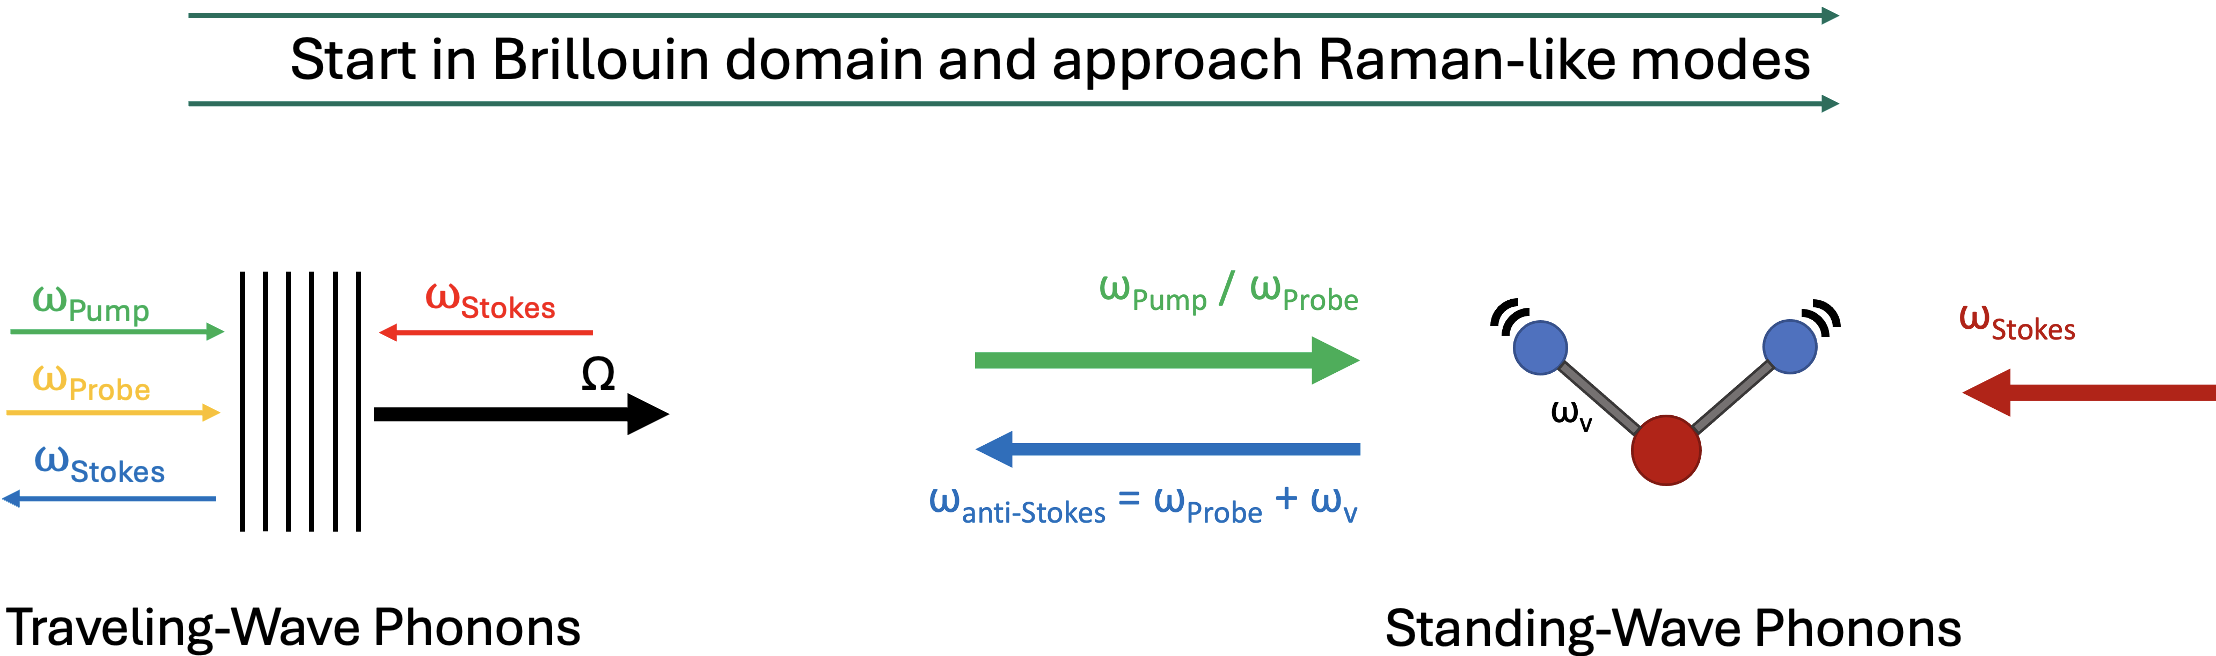
\includegraphics[width=\textwidth]{figs/4-Raman/ExploreBrillouinRamanTransition.png}
  \caption{Transition from Brillouin domain to Raman-like modes.}
  \label{fig:Raman:BrillouinRamanTransition}
\end{figure}

\begin{figure}[t]
  \centering
  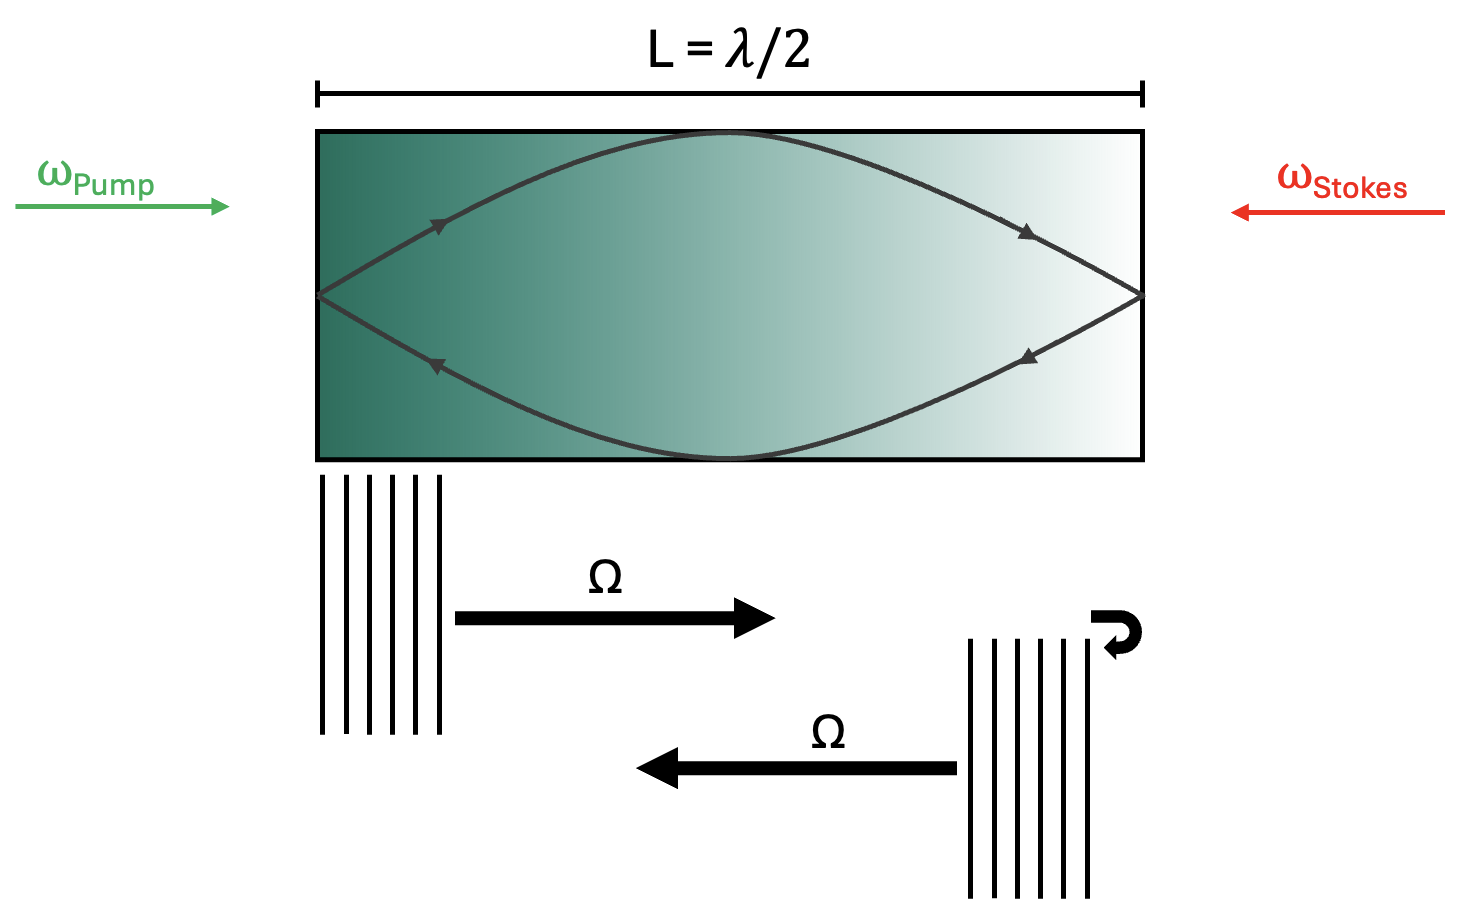
\includegraphics[width=.85\textwidth]{figs/4-Raman/GeometryDeterminesFundamentalFreq.png}
  \caption{Geometry determines fundamental frequency.}
  \label{fig:Raman:GeometryDeterminesFundamentalFreq}
\end{figure}

\subsection{Acousto-Optic Response of Materials}
\label{subsec:Raman:Acousto-OpticResponse}

\begin{figure}[t]
  \centering
  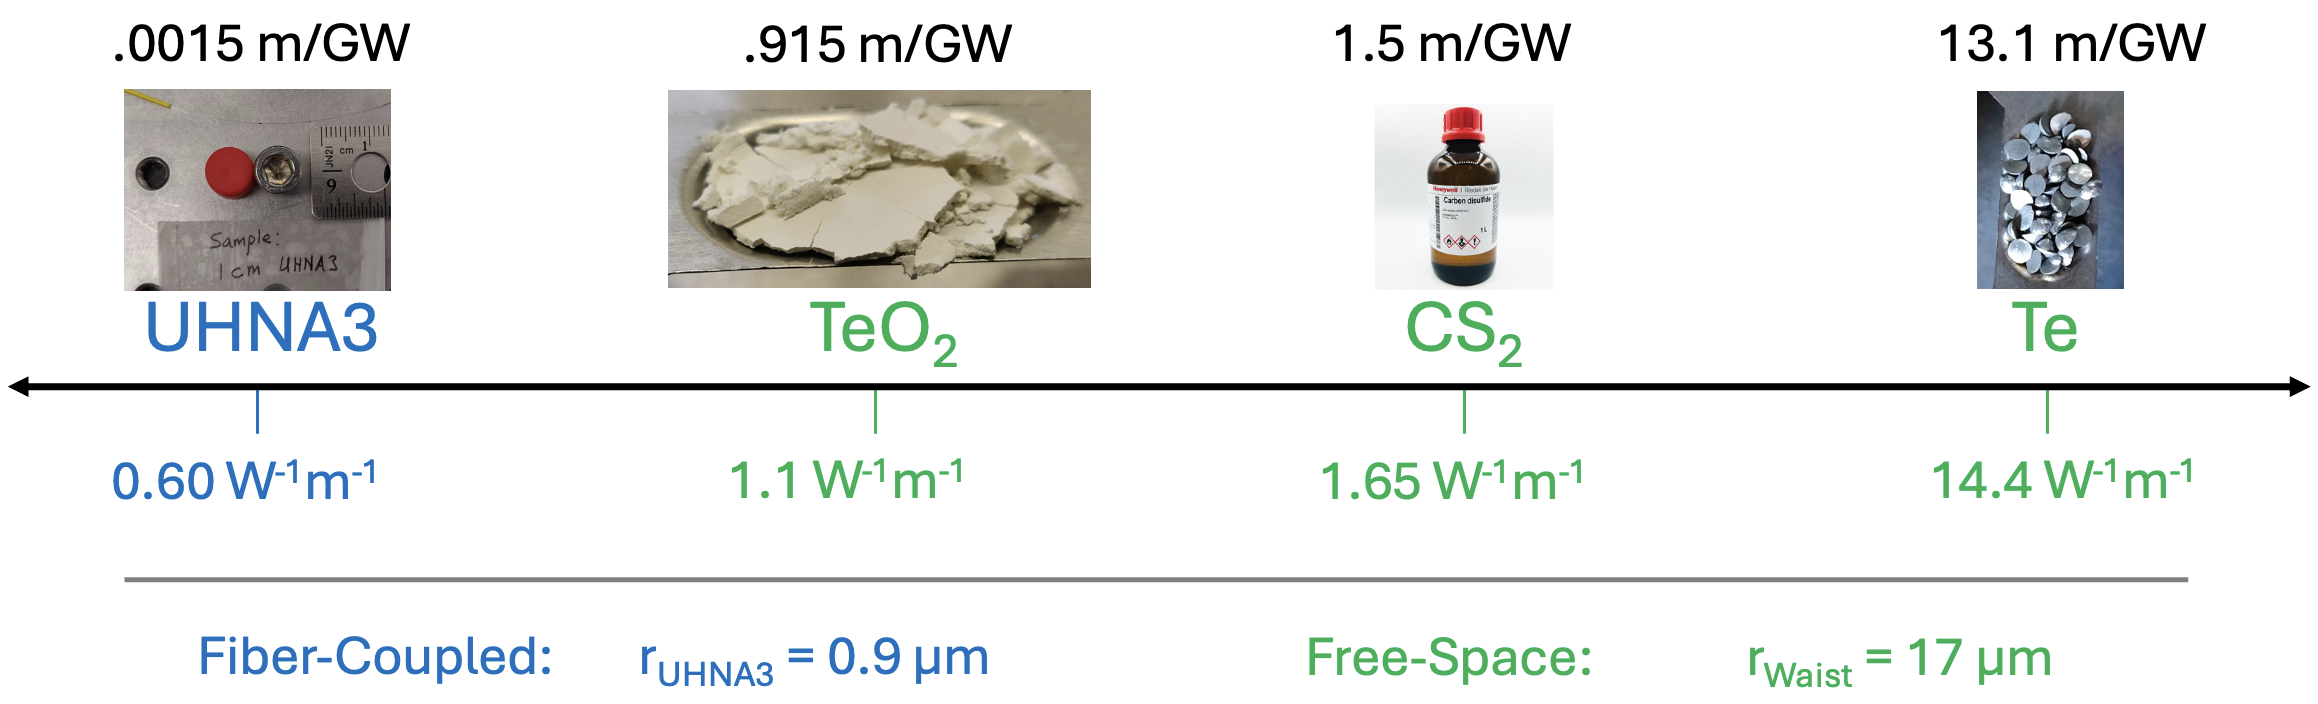
\includegraphics[width=\textwidth]{figs/4-Raman/GainOfRelevantMaterials.png}
  \caption{Gain of relevant materials.}
  \label{fig:Raman:GainOfRelevantMaterials}
\end{figure}

\subsection{Phonon Mean Travel Distance}
\label{subsec:Raman:PhononMeanTravelDistance}

phonon mean travel distance

\subsection{Acoustic Impedance and Reflection}
\label{subsec:Raman:AcousticImpedanceAndReflection}

\begin{figure}[t]
  \centering
  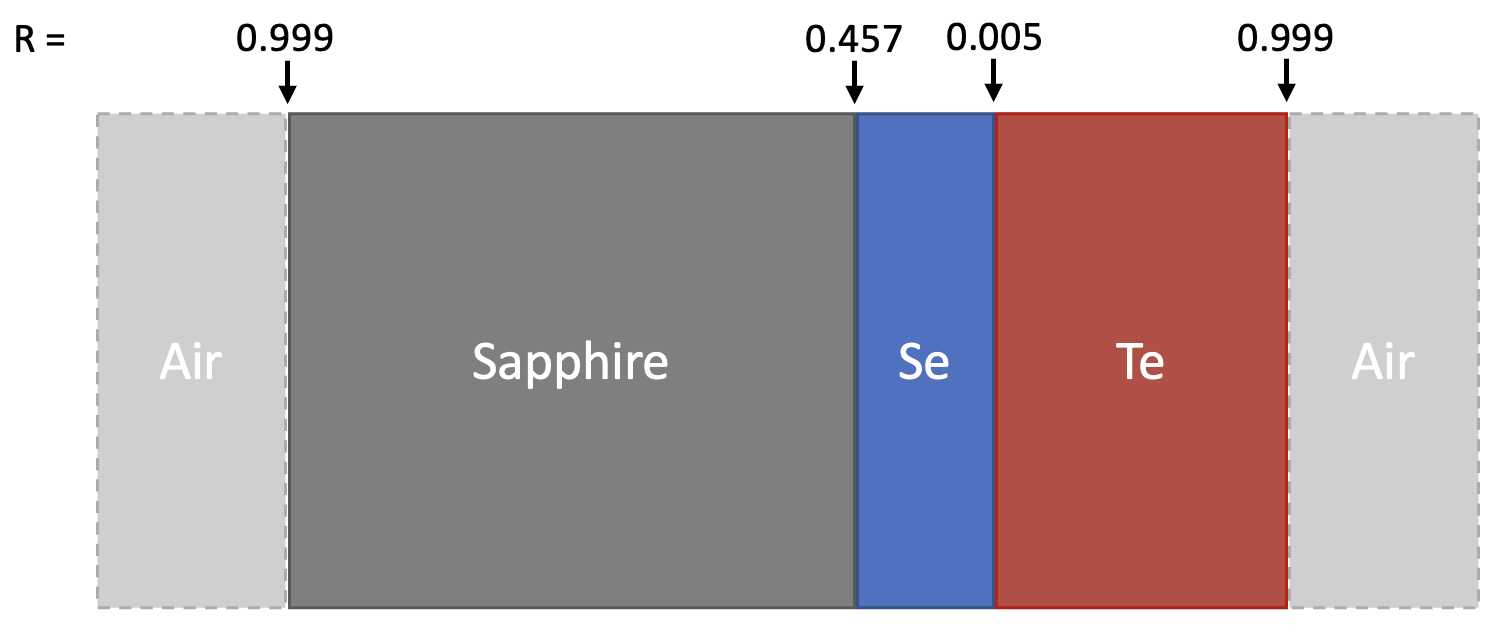
\includegraphics[width=\textwidth]{figs/4-Raman/AcousticImpedance.png}
  \caption{Acoustic impedance.}
  \label{fig:Raman:AcousticImpedance}
\end{figure}

%--------------------------------------------------------------------%

\section{Target Platform Evolution and Collaborative Fabrication}
\label{sec:Raman:TargetPlatforms}

\subsection{Germanium-Doped Optical Fiber}
\label{subsec:Raman:Target:UHNA3}

1cm -> 1mm

\begin{figure}[t]
    \centering
    \begin{subfigure}[b]{0.49\textwidth}
        \centering
        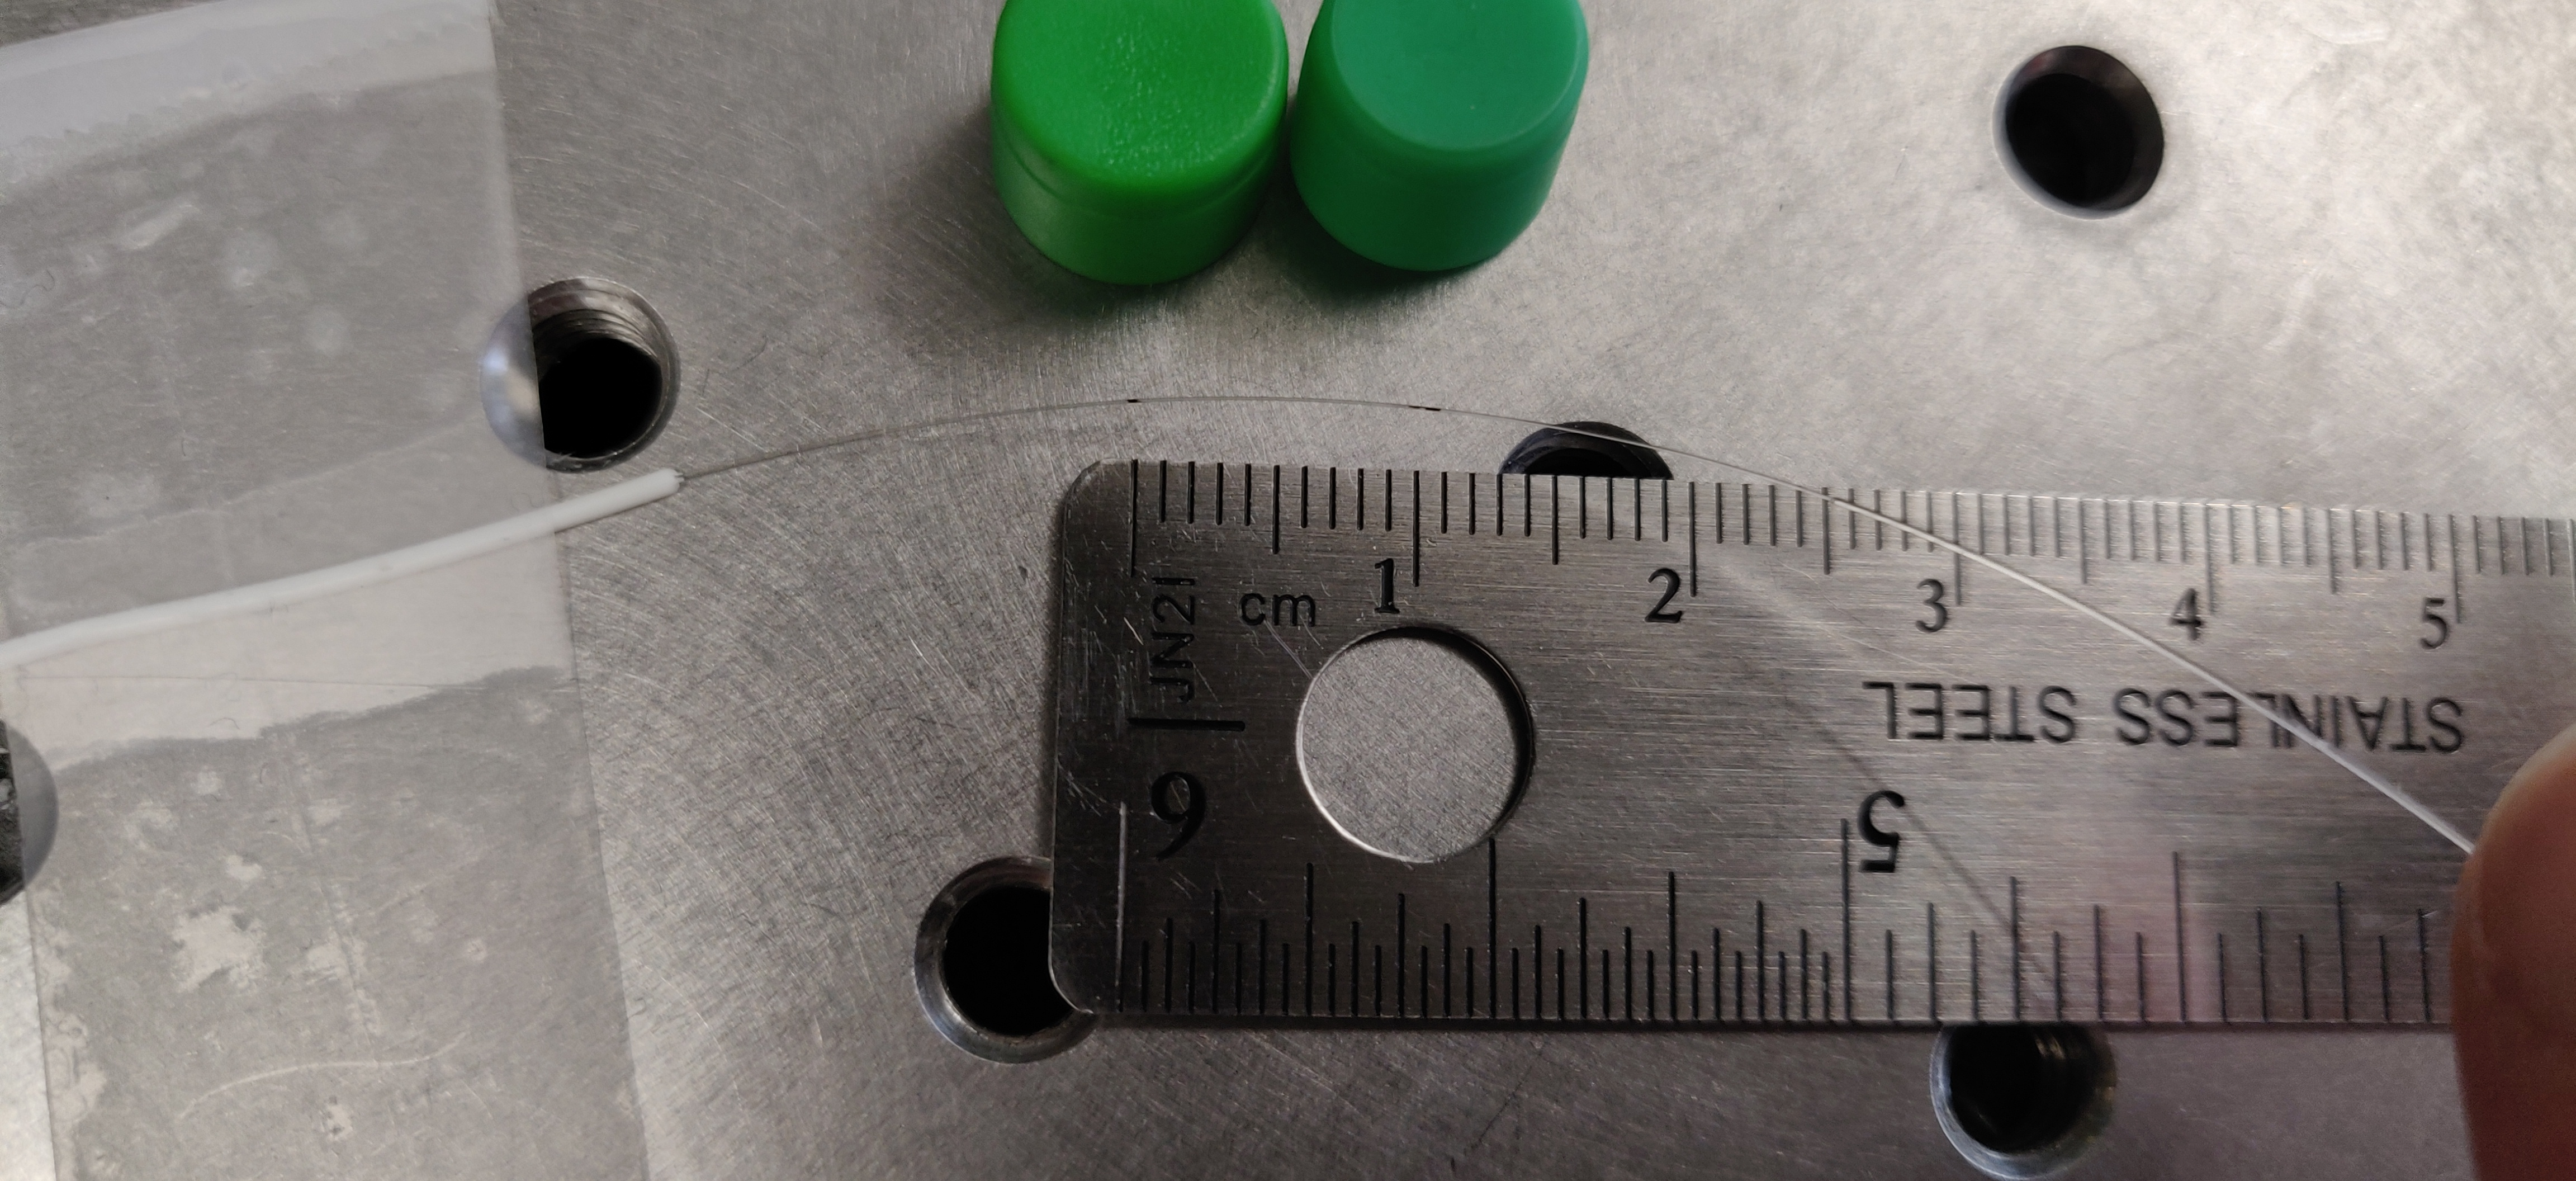
\includegraphics[width=\textwidth]{figs/4-Raman/1cm UHNA3.jpeg}
        \caption{}
        \label{fig:Raman:1cmUHNA3pic}
    \end{subfigure}
    \hfill
    \begin{subfigure}[b]{0.49\textwidth}
        \centering
        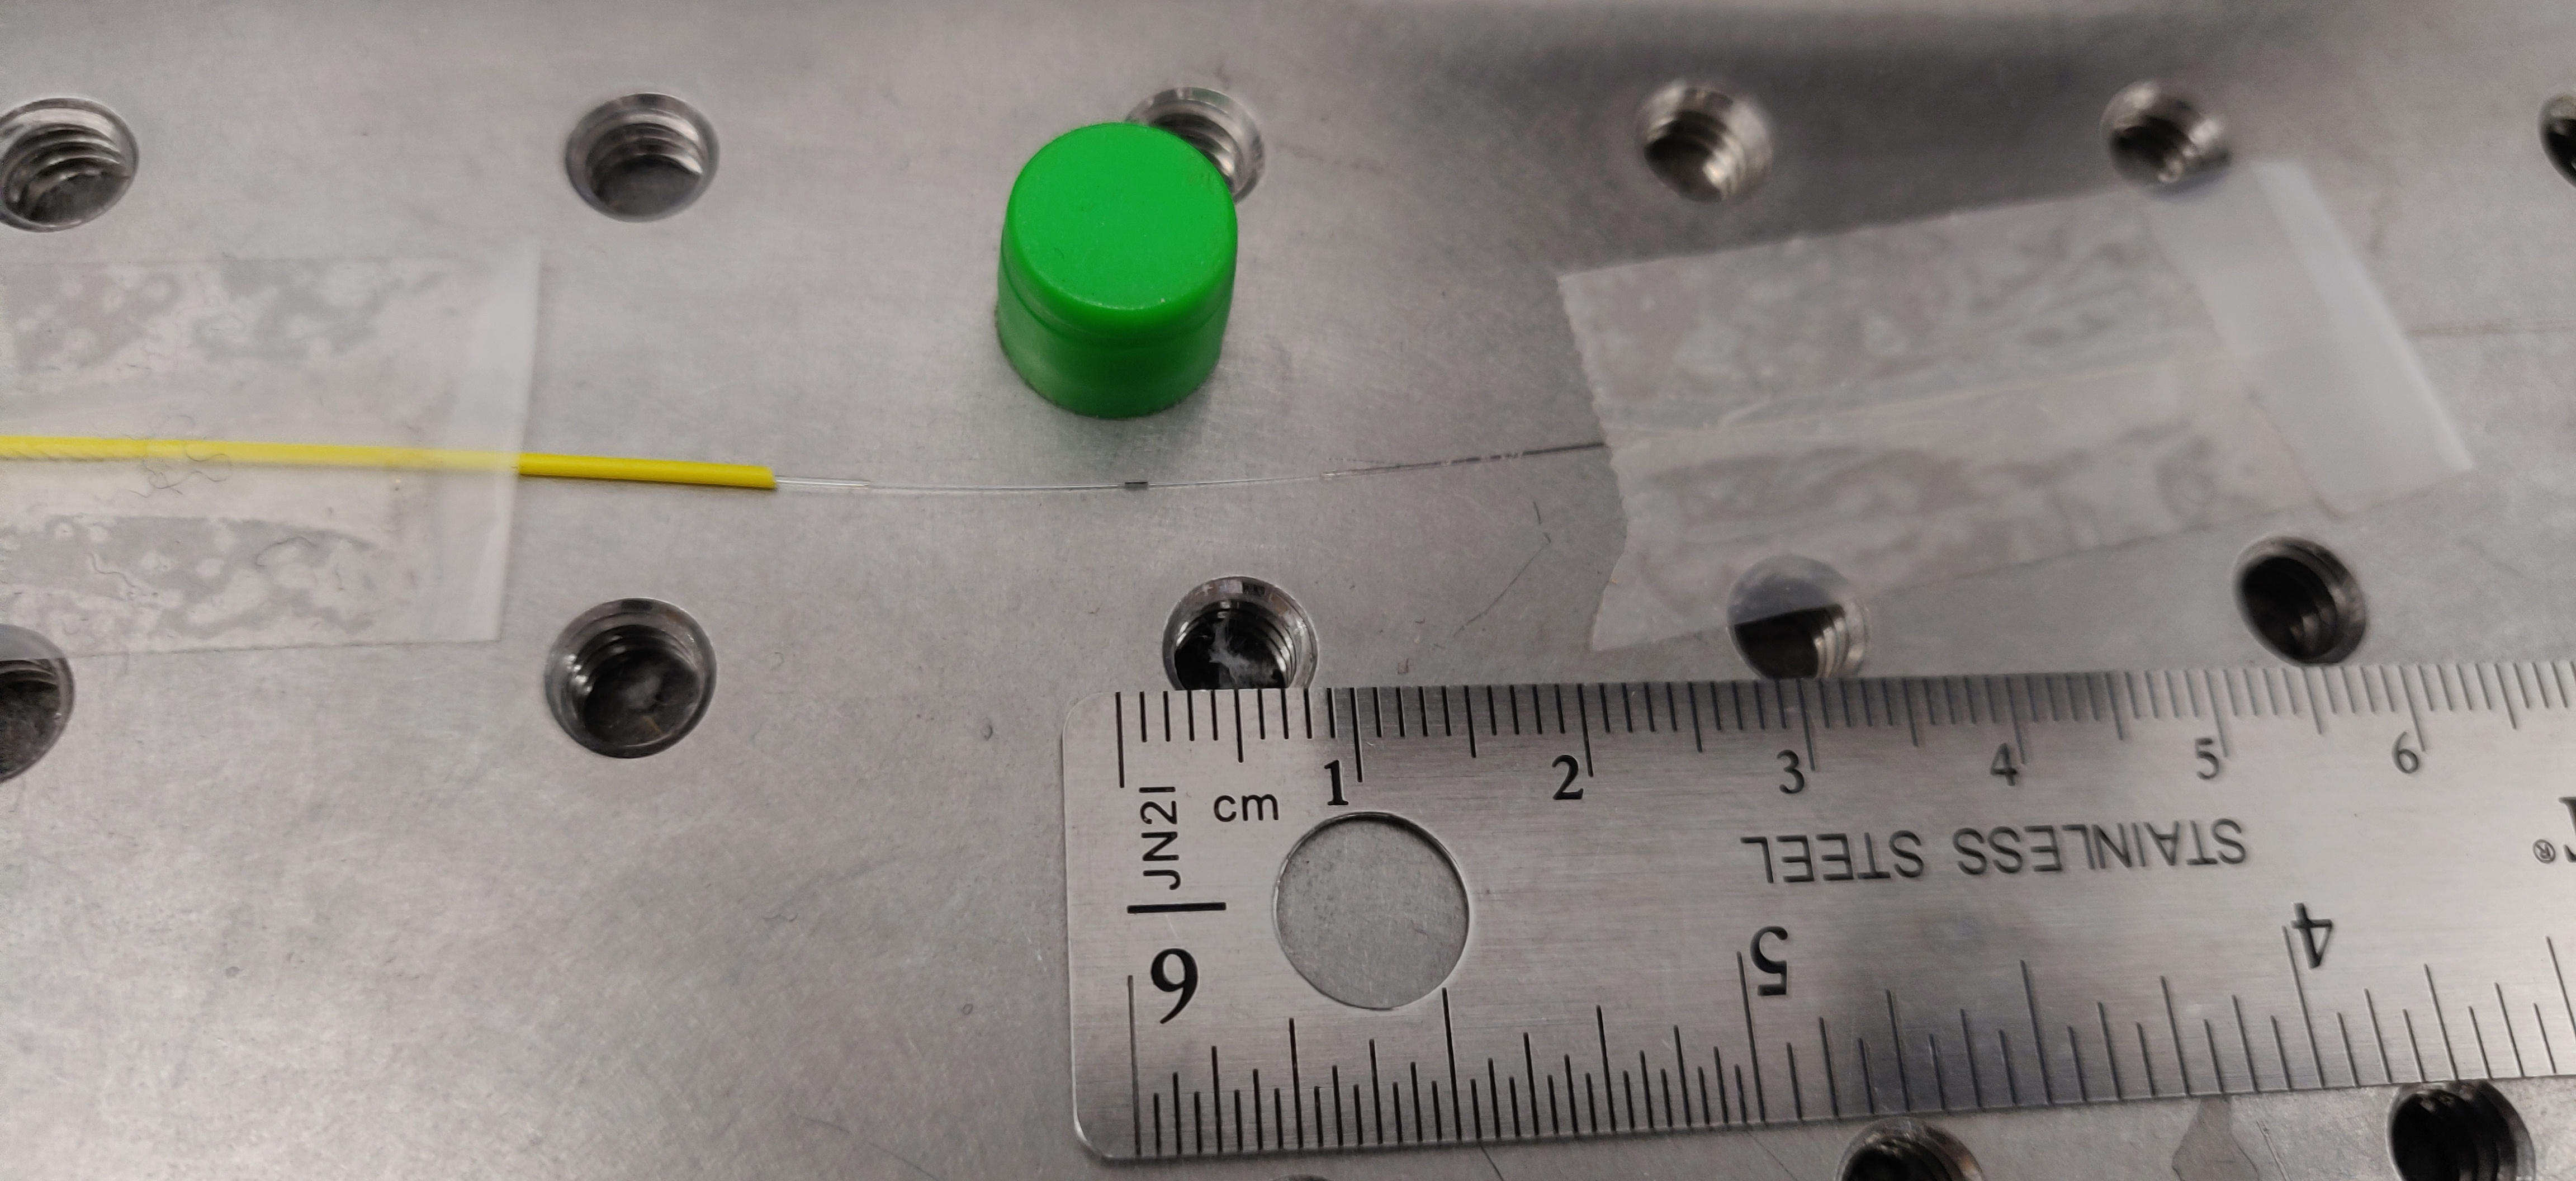
\includegraphics[width=\textwidth]{figs/4-Raman/1mm UHNA3 in apparatus.jpeg}
        \caption{}
        \label{fig:Raman:1mmUHNA3pic}
    \end{subfigure}
    \caption{\SI{1}{\centi\meter} (\ref{fig:Raman:1cmUHNA3pic}) and \SI{1}{\milli\meter} (\ref{fig:Raman:1mmUHNA3pic}) \ac{UHNA3}.}
    \label{fig:Raman:UHNA3}
\end{figure}

\subsection{Free-Space Optics with Liquid Carbon Disulfide}
\label{subsec:Raman:Target:CS2Vial}

Free space with vial

\begin{figure}[t]
    \centering
    \begin{subfigure}[b]{0.49\textwidth}
        \centering
        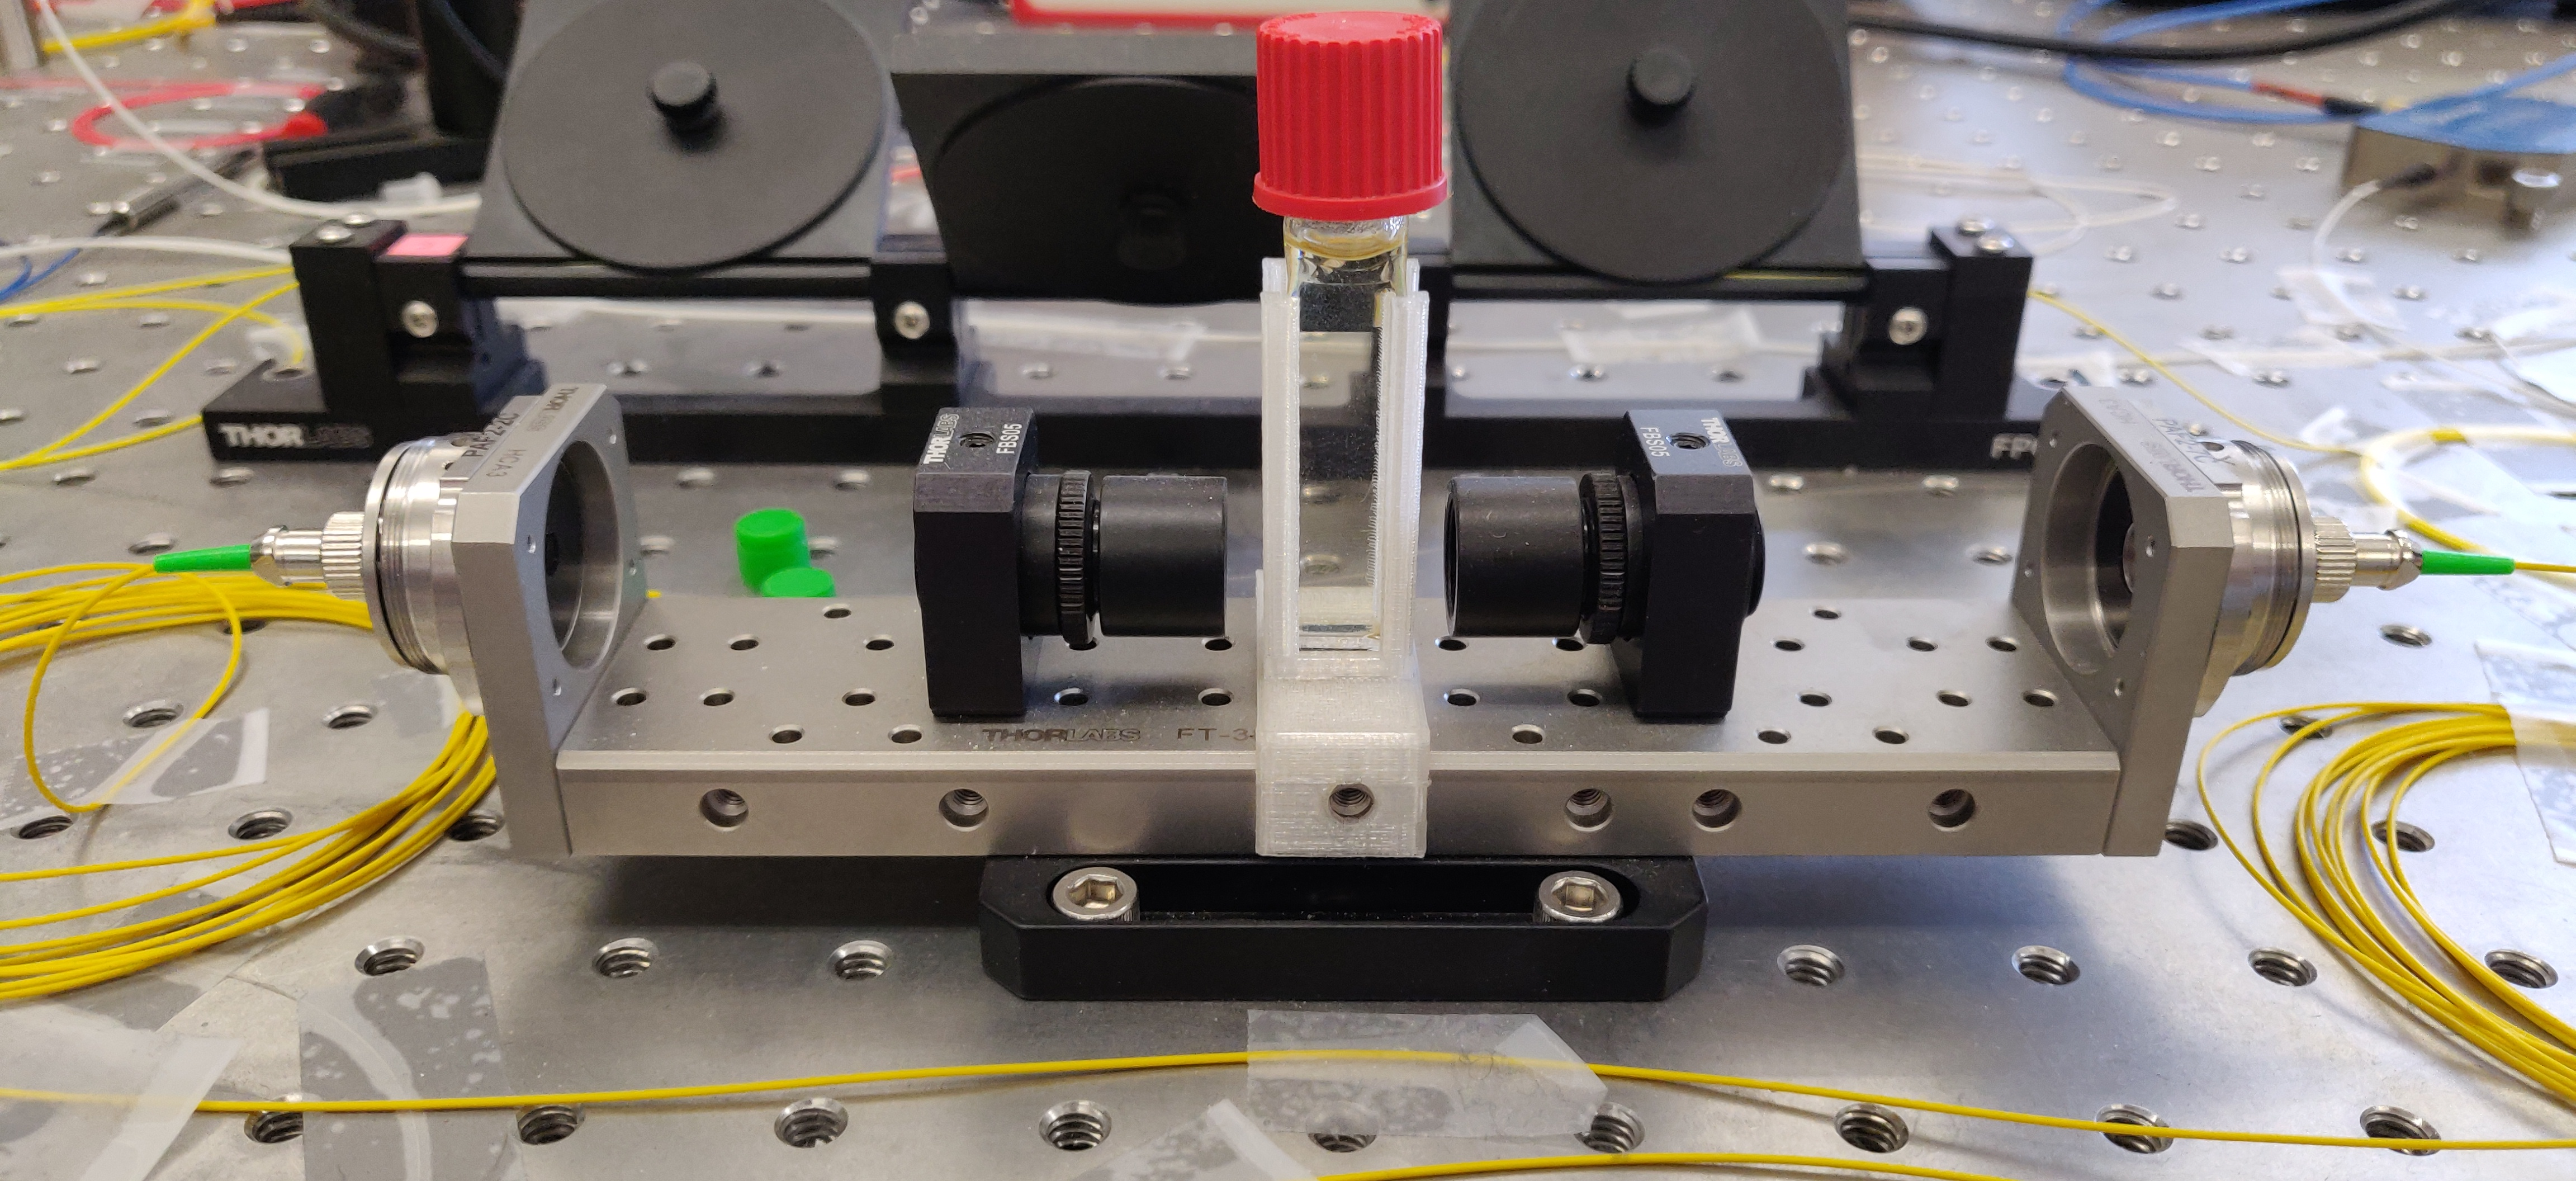
\includegraphics[width=\textwidth]{figs/4-Raman/1cmCS2.jpeg}
        \caption{}
        \label{fig:Raman:1cmCS2}
    \end{subfigure}
    \hfill
    \begin{subfigure}[b]{0.49\textwidth}
        \centering
        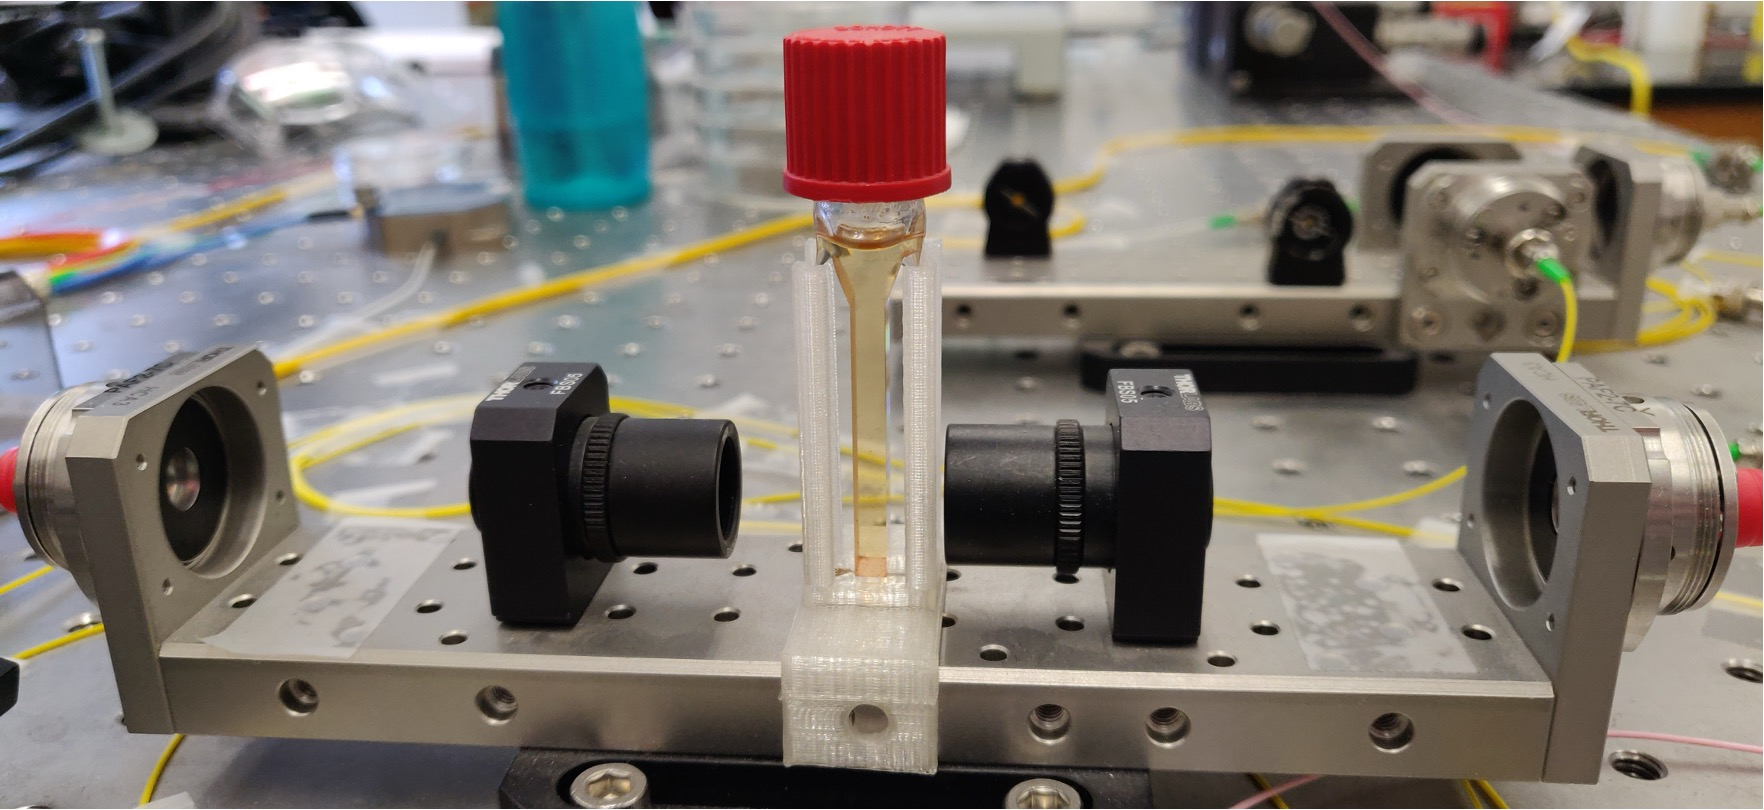
\includegraphics[width=\textwidth]{figs/4-Raman/4mmCS2.jpg}
        \caption{}
        \label{fig:Raman:4mmCS2}
    \end{subfigure}
    \caption{\SI{1}{\centi\meter} (\ref{fig:Raman:1cmCS2}) and \SI{4}{\milli\meter} (\ref{fig:Raman:4mmCS2}) liquid \ce{CS2}.}
    \label{fig:Raman:CS2Cuvet}
\end{figure}

\subsection{Tellurium Dioxide Thin Film}
\label{subsec:Raman:Target:TeO2}

Gibbs collab -> dissolve, sheet music

\begin{figure}[t]
  \centering
  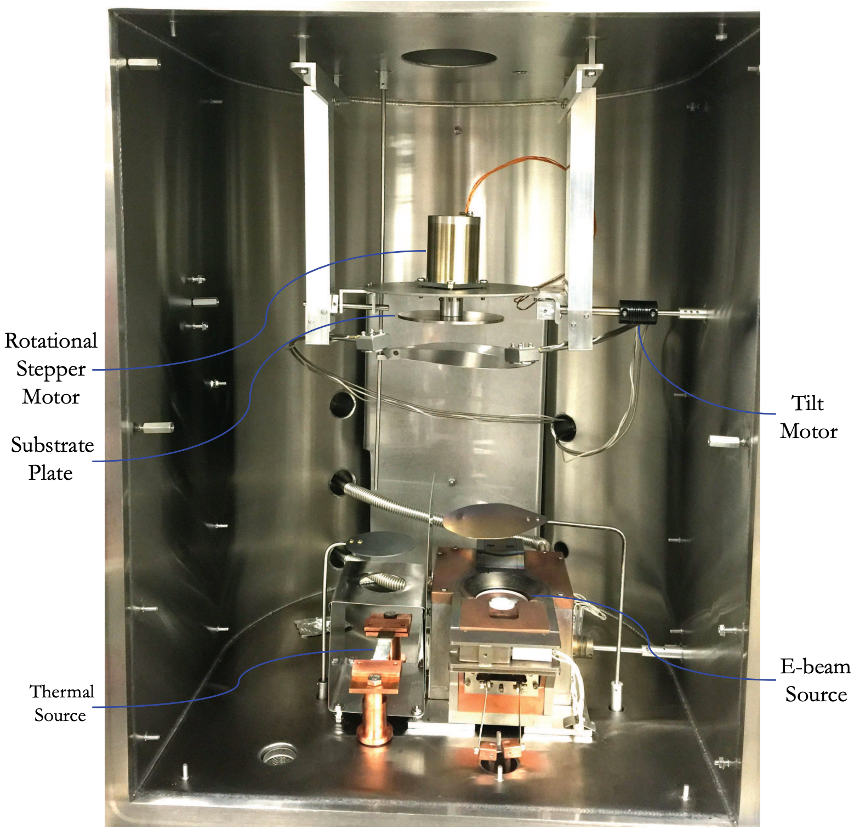
\includegraphics[width=\textwidth]{figs/4-Raman/DepositionChamber.png}
  \caption{John Gibbs Nanotechnology Laboratory \ac{PVD} chamber.}
  \label{fig:Raman:DepositionChamber}
\end{figure}

\begin{figure}[t]
  \centering
  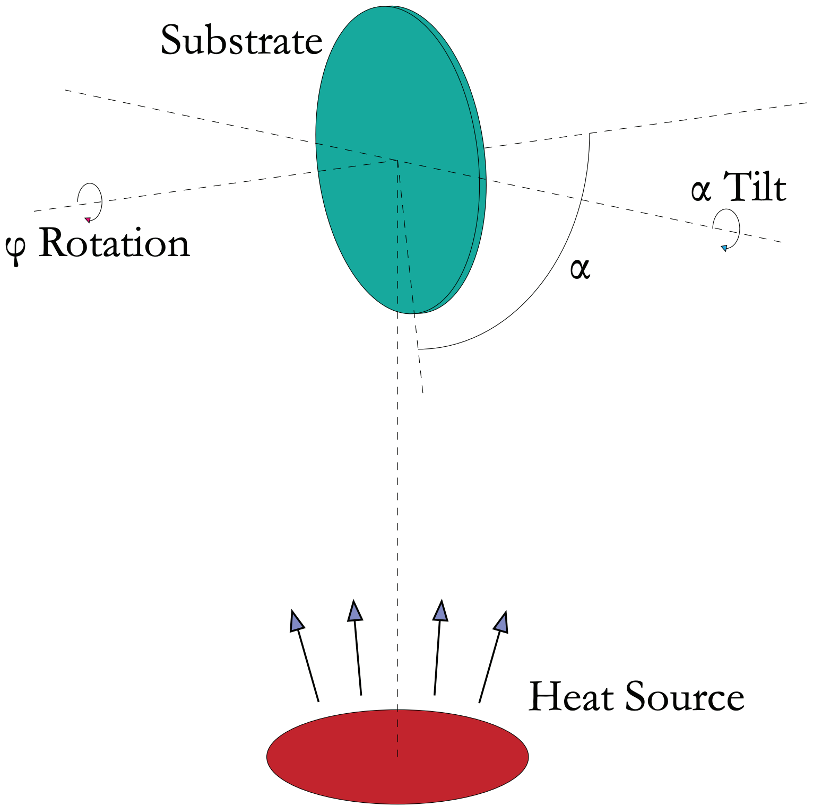
\includegraphics[width=\textwidth]{figs/4-Raman/GLAD.png}
  \caption{Diagram showing Glancing Angle Deposition (\acs{GLAD}). This technique offer the ability to fabricate complex nanosgeometries such as rods and helices via programatic control of deposition parameters and substrate degrees of freedom.}
  \label{fig:Raman:GLAD}
\end{figure}

\subsection{Tellurium Thin Film}
\label{subsec:Raman:Target:Te}

Gibbs collab -> CINT collab -> oxidizes to TeO2

\begin{figure}[t]
    \centering
    \begin{subfigure}[b]{0.49\textwidth}
        \centering
        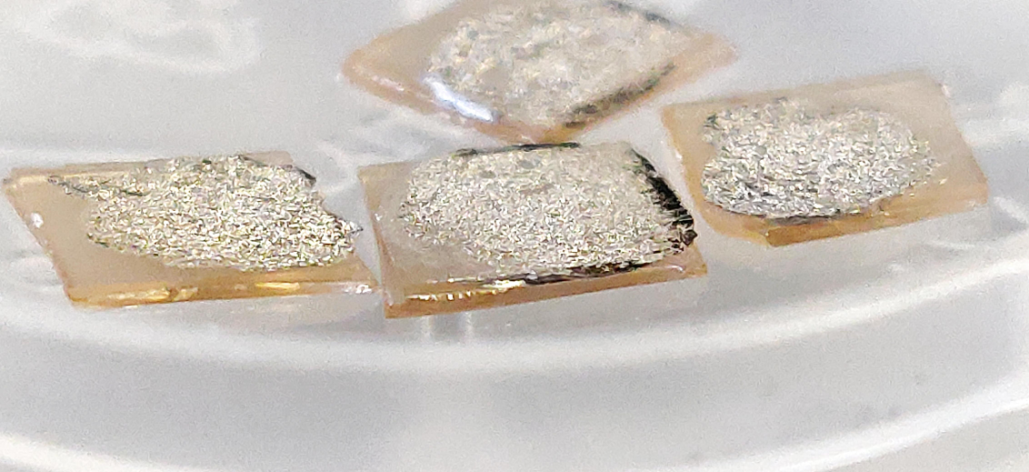
\includegraphics[width=\textwidth]{figs/4-Raman/CINTSamples.png}
        \caption{}
        \label{fig:Raman:CINTSamplesFacedown}
    \end{subfigure}
    \hfill
    \begin{subfigure}[b]{0.49\textwidth}
        \centering
        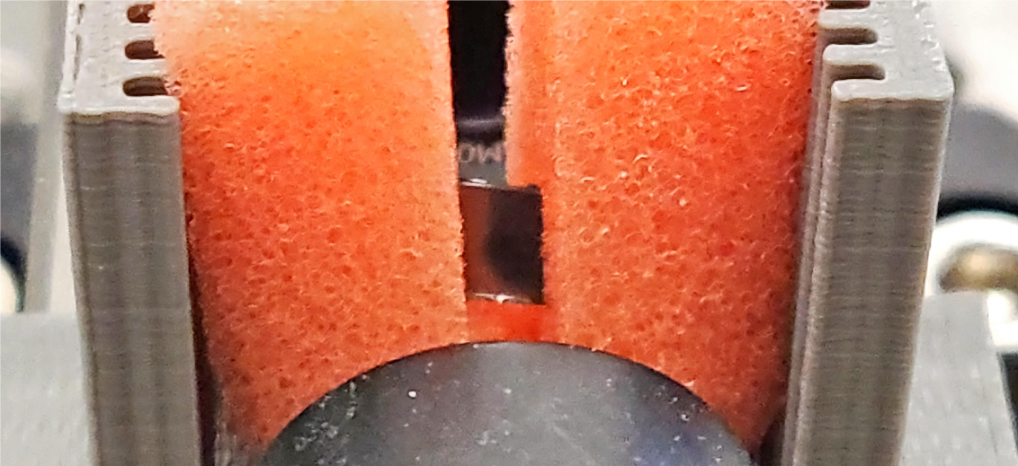
\includegraphics[width=\textwidth]{figs/4-Raman/TeCINTinFoam.png}
        \caption{}
        \label{fig:Raman:TeCINTinFoam}
    \end{subfigure}
    \caption{(\ref{fig:Raman:CINTSamplesFacedown}) Photograph of sapphire substrates primed with \SI{20}{\nano\meter} \ce{Se} adhesion layer. Critical surface is layed face down in curved-bottom protective container. (\ref{fig:Raman:TeCINTinFoam}) \SI{500}{\nano\meter} \ce{Te} thin film sample secured in beam path of \acl{CoBS}. \ce{Te} is deposited ontop of the \SI{20}{\nano\meter} \ce{Se} adhesion layer for ablation prevention.}
    \label{fig:Raman:CINTSamples}
\end{figure}

\subsection{Carbon Disulfide Micrometer Cell}
\label{subsec:Raman:Target:CS2Cells}

cells -> 1 W amp, bubble test

\subsection{Suspended Silica Rib Waveguide}
\label{subsec:Raman:Target:Waveguide}

BYU collab -> initial test took 9 months to learn and measure

\subsection{Elastically-Suspended Photonic-Phononic Waveguide}
\label{subsec:Raman:Target:WigglyWaveguide}

BYU collab - proof of fabrication: holes and trampoline

%--------------------------------------------------------------------%

\section{Results}
\label{sec:Raman:Results}

UHNA3 - 1cm, 1mm
CS2 vial - 4mm, 2mm
TeO2 films - 1um, 500nm
CS2 - 1mm, 100um, (10um not quite)
chip waveguide - chip/nochip, holes

\begin{figure}[t]
  \centering
  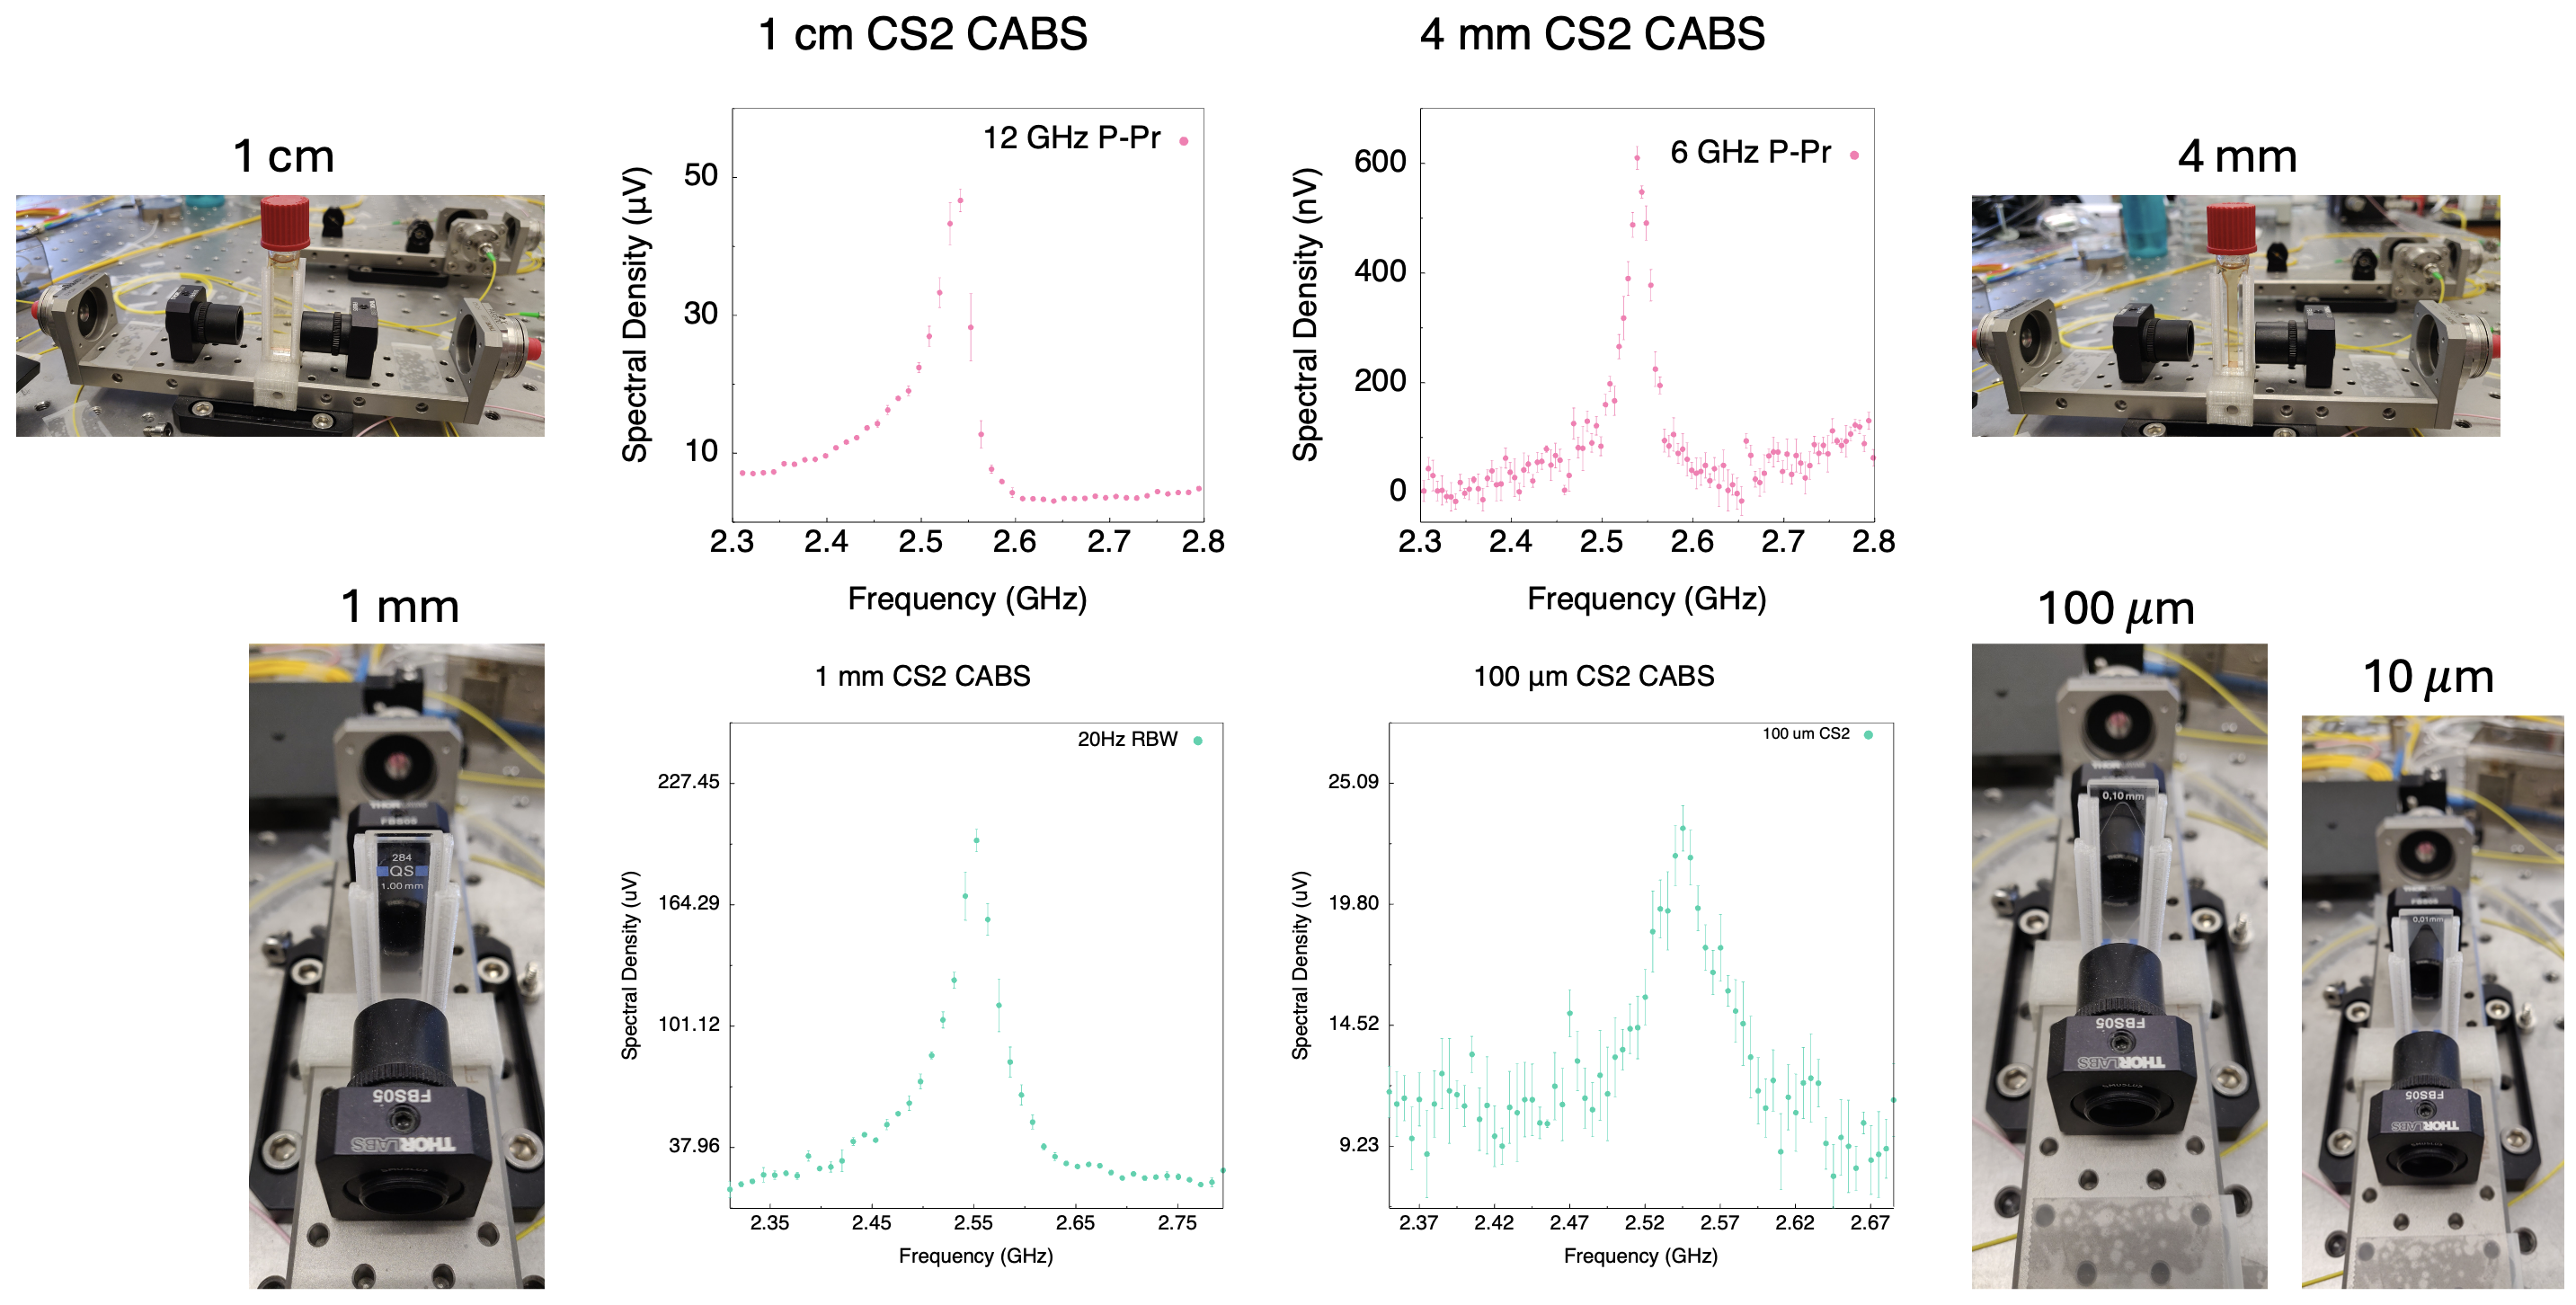
\includegraphics[width=\textwidth]{figs/4-Raman/StartBigApproachSmall.png}
  \caption{Start big, approach small.}
  \label{fig:StartBigApproachSmall}
\end{figure}

\begin{figure}[t]
  \centering
  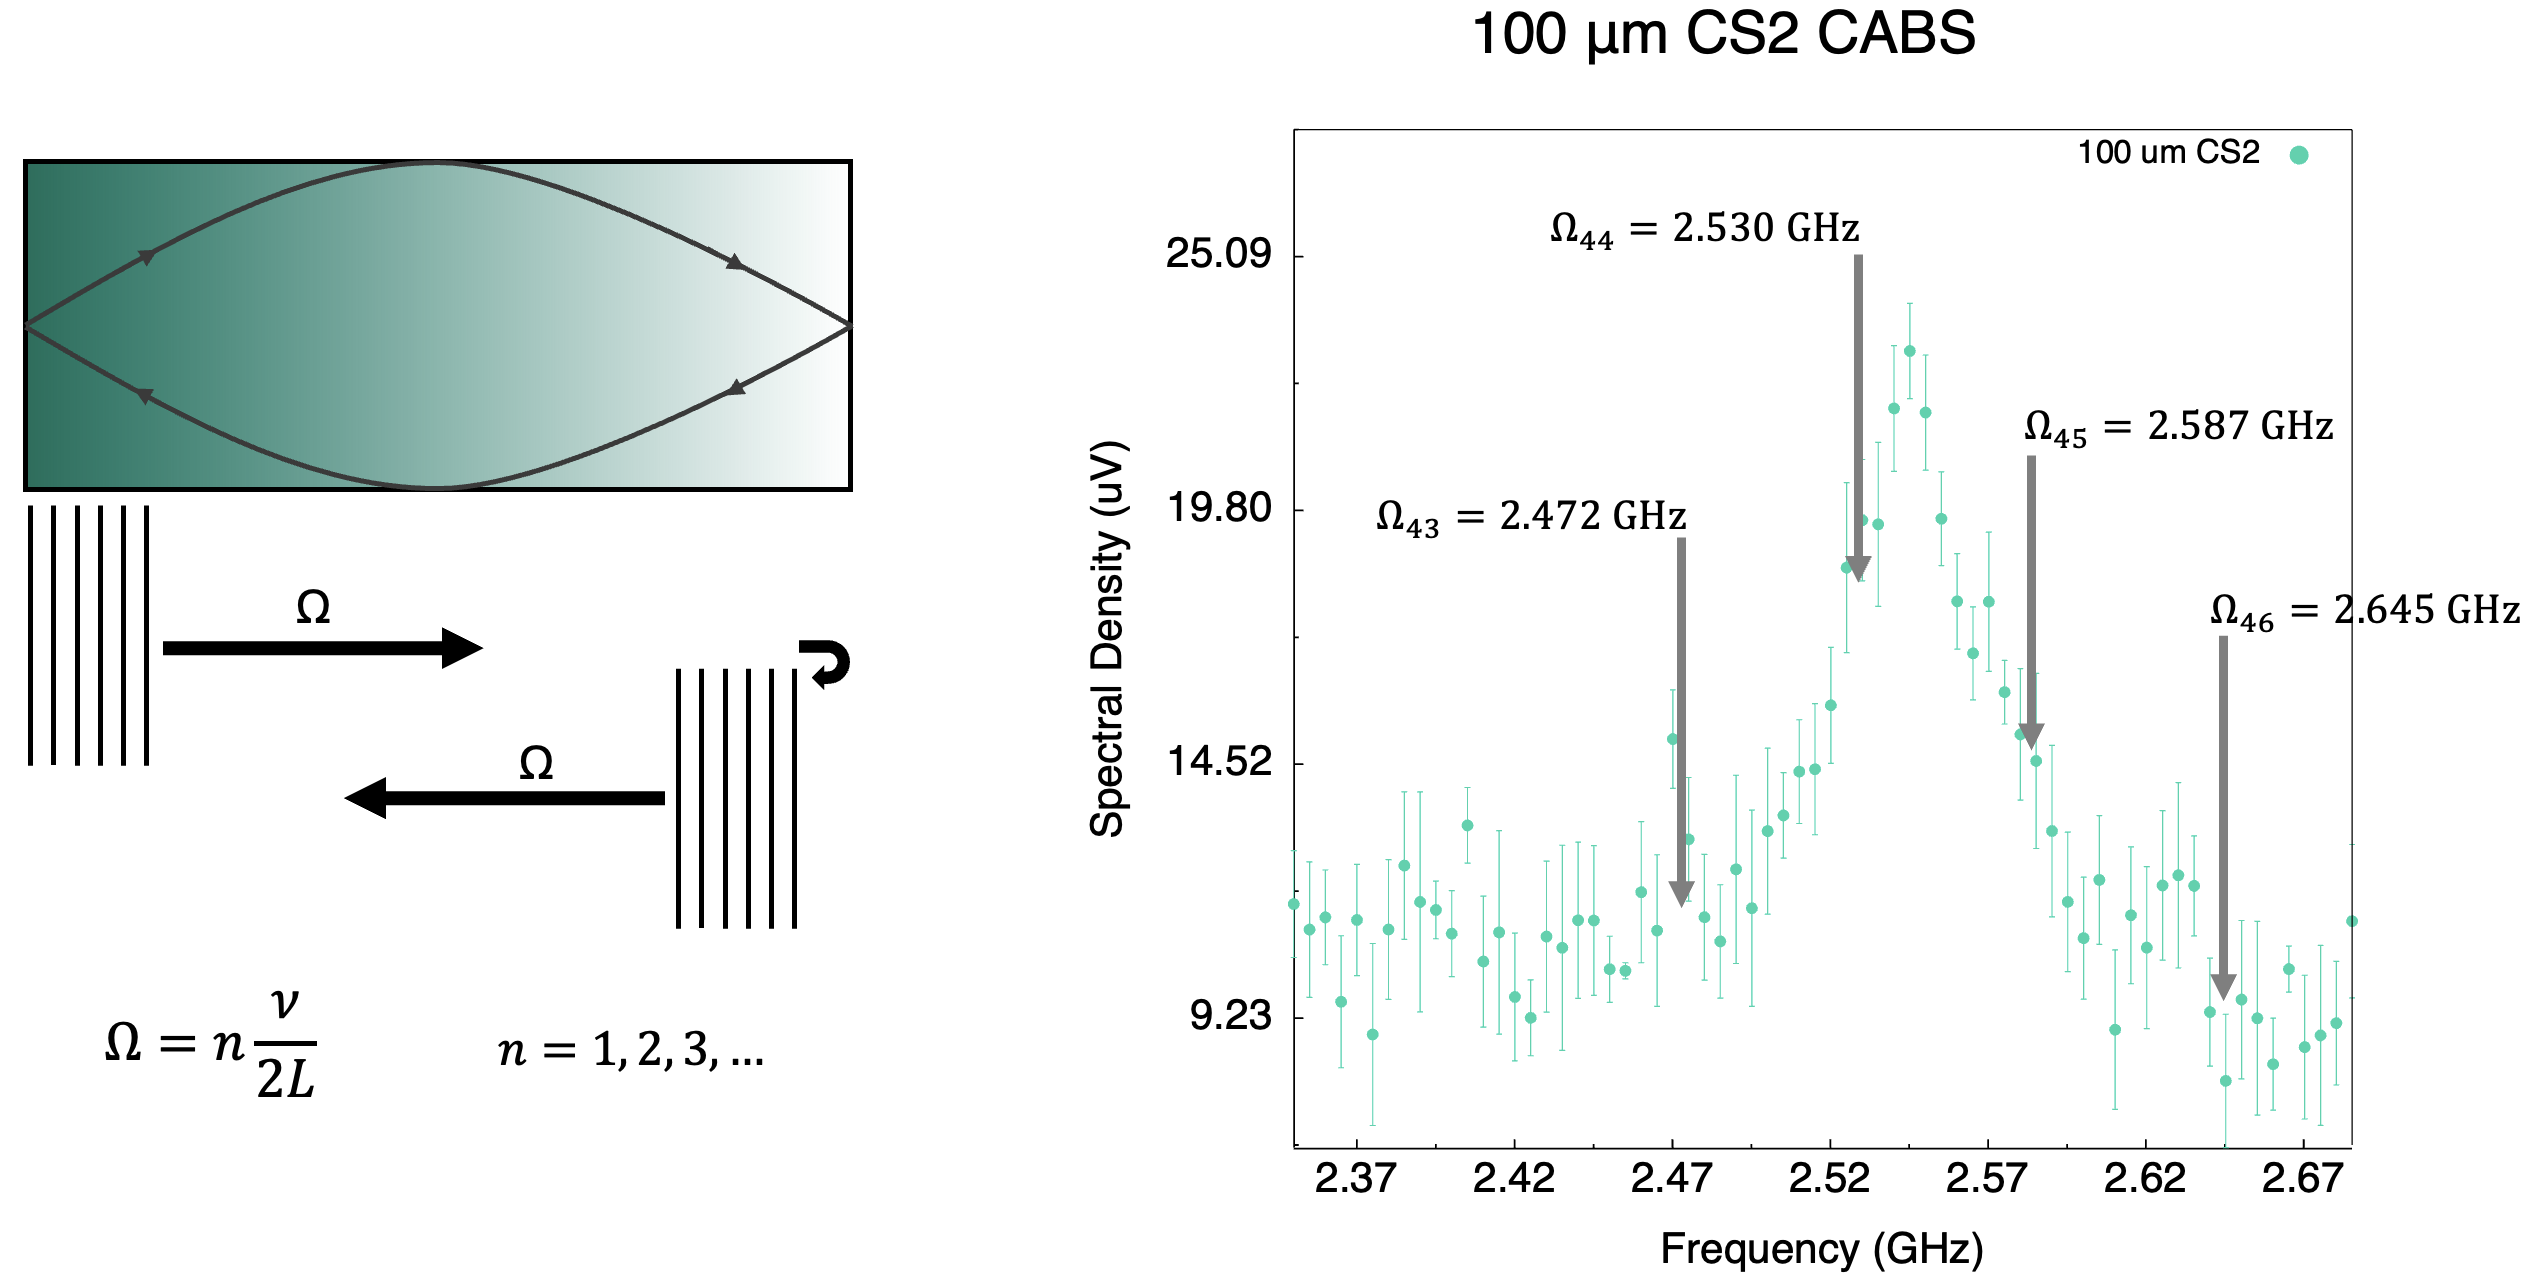
\includegraphics[width=\textwidth]{figs/4-Raman/HowWouldRamanModesAppear.png}
  \caption{How would Raman modes appear.}
  \label{fig:HowWouldRamanModesAppear}
\end{figure}

%--------------------------------------------------------------------%

\section{Discussion}
\label{sec:Raman:Discussion}

\subsection{Pathways to Brillouin-Induced Raman Modes}
\label{subsec:Raman:Pathways}
Ideal platforms by category
  waveguide - long TeO2 rib, evenly spaced square holes
  TeO2 thin film/crystal - dissolve only small area of substrate for beam spot
  CS2 cell - 5um
  Fiber - notched, acoustic fiber Bragg grating

\subsection{Conclusion}
\label{subsec:Raman:Conclusion}


\clearpage
\thispagestyle{empty}
\null
\newpage
